\chapter{Full and Reduced Inventory-Control Equations}\label{ch:control}
The lift makes a finite-state description available, but its control PDE can still be too large. We retain the common cash--inventory mechanism, declare terminal liquidation and admissible quote bounds, and compare a scalar surrogate with its immersion in the full factor state. Multi-asset coupling is introduced here at the level of the model; its performance is assessed in the common results chapter.
\section{Full Lifted Rough-Volatility HJB}


\subsection{State dynamics and objective}
Take positive decay rates $\lambda_i$ and deterministic weights $w_i$. The inherited finite-factor benchmark is
\[
 dZ_t^{(i)}=-\lambda_i Z_t^{(i)}dt+dB_t,\qquad
 Y_t=\sum_{i=1}^M w_iZ_t^{(i)},\qquad
 dS_t=\sqrt{v(Y_t)}\,dW_t,
\]
where the same Brownian motion $B$ drives every factor and $W$ is independent of $B$. Thus the instantaneous factor covariance is $\mathbf1\mathbf1^\top$, not the identity. Under stationary initialization,
\[
 \Sigma_{ij}=\frac1{\lambda_i+\lambda_j},\quad
 s_Y^2=w^\top\Sigma w,\quad
 v(y)=\sigma_0^2\exp\!\left(\beta y-\tfrac12\beta^2s_Y^2\right).
\]
The exact one-step innovation covariance is
\[
 Q_{ij}(h)=\frac{1-\exp[-(\lambda_i+\lambda_j)h]}{\lambda_i+\lambda_j}.
\]
Independent factors would represent a different model. The finite exponential mixture is a benchmark approximation; this draft does not establish a calibrated power-law limit or a Hurst-parameter interpretation beyond the inherited weight rule.

Inventory $q\in\{-Q,\ldots,Q\}$ changes by one unit on a fill. Bid and ask offsets $\delta^b,\delta^a$ have arrival intensities $A e^{-k\delta}$. At the inventory limits, the side that would violate the constraint is disabled. The terminal cash-equivalent liquidation cost is
\[
 L(q,y)=(\ell_1+\ell_v\sqrt{v(y)})|q|+\ell_2q^2.
\]
The objective is exponential utility of terminal marked-to-market wealth less $L$, with risk aversion $\gamma>0$. Under price translation invariance and independent price/factor noise, use
\[
 U(t,x,s,q,z)=-\exp\{-\gamma[x+qs+\theta(t,q,z)]\},
 \qquad \theta(T,q,z)=-L(q,w^\top z).
\]
Here $U$ is utility and $\theta$ is a certainty-equivalent adjustment. Applying the nonlinear operator to one while interpreting it as the other would change the residual.

\subsection{The operator and bounded controls}
Set $b_i(z)=-\lambda_i z_i$, $a=\mathbf1\mathbf1^\top$, and
\[
 h(d)=\max_{\delta\in[\delta_{\min},\delta_{\max}]}
 \frac{A e^{-k\delta}}\gamma\left[1-e^{-\gamma(\delta+d)}\right].
\]
The maximizing quote, for this declared admissible interval, is
\[
 \delta^*(d)=\operatorname{clip}\!\left(
 \frac{\log(1+\gamma/k)}\gamma-d,
 \delta_{\min},\delta_{\max}\right).
\]
Substitution of the utility ansatz into the diffusion and jump generator yields
\begin{align*}
 \mathcal H_F[\theta]={}&\theta_t+b^\top\nabla\theta
 +\tfrac12\operatorname{tr}(a\nabla^2\theta)
 -\tfrac\gamma2\nabla\theta^\top a\nabla\theta
 -\tfrac\gamma2q^2v(w^\top z)\\
 &+\mathbf1_{q<Q}h(\theta(t,q+1,z)-\theta(t,q,z))\\
 &+\mathbf1_{q>-Q}h(\theta(t,q-1,z)-\theta(t,q,z)).
\end{align*}
The equation is $\mathcal H_F[\theta]=0$. The negative gradient-square term comes from differentiating the exponential utility ansatz. The common factor driver requires all mixed Hessian entries. If price/factor correlation is introduced later, additional cross terms must be derived before reusing this operator.

The inherited HFT2 solver uses an unconstrained arrival Hamiltonian and clips evaluated quotes afterwards. The present diagnostic uses the bounded Hamiltonian on both sides of the residual comparison, with interval $[0.02,4]$. It therefore evaluates a declared admissible-control problem rather than silently identifying the two implementations. The positive transformed baseline below uses the bounded Hamiltonian consistently; the historical clipped results remain a separate configuration.
\section{Lift calibration across the three Hurst regimes}

The numerical comparison is run for
\[
H=0.2,\qquad H=0.5,\qquad H=0.8.
\]
In interpretive terms, these correspond respectively to an anti-persistent or locally mean-reverting-like regime, the standard Brownian-labelled lift, and a persistent or trend-following-like regime. The Markovian lifting uses the same six-factor grid in every case,
\[
M=6,
\qquad
\lambda=(3.0,\ 6.80,\ 15.43,\ 35.00,\ 79.37,\ 180.0),
\]
while the weights change with \(H\) through the power-law prescription
\[
w_k \propto \lambda_k^{-(H+1/2)}.
\]
As \(H\) increases, more weight shifts toward the slow factors. This is exactly what one should expect: the persistent regime keeps more memory in the low-frequency components, whereas the anti-persistent regime places relatively more mass on faster adjustments.

The full lift remains vector-valued, but the HJB is solved on a reduced scalar surrogate \(Y_t\). In the numerical implementation, the stationary variance of the lift is matched exactly, while the reduced mean-reversion scale used inside the HJB grid is kept common across the three runs at
\[
\kappa_Y=1.35.
\]
This is a deliberate modeling choice. It prevents the surface comparison from being dominated by the compression step itself, while still allowing \(H\) to alter the variance map and the persistence diagnostics of the lifted environment. The forward simulations, however, do \emph{not} collapse back to the same scalar OU path: they use the full lifted OU stack and only then aggregate it into the volatility driver. The induced local variance remains
\[
v_t
=
\sigma_0^2
\exp\!\left(
\beta Y_t
-\frac12\beta^2\Var(Y_\infty)
\right),
\]
with \(\sigma_0=1.1\) and \(\beta=0.75\), so that the traded mid-price follows
\[
dS_t=\sqrt{v_t}\,dW_t^S.
\]

Table~\ref{hft2-tab:hjb_calibration} summarizes the lift calibration. The monotone increase in \(\Var(Y_\infty)\) and in the lag-one autocorrelation makes the interpretation clear: the case \(H=0.2\) is the roughest and most reversal-prone, \(H=0.5\) is the benchmark, and \(H=0.8\) is the most persistent.

\begin{table}[H]
\centering
\caption{Markovian-lifting calibration used in the three numerical regimes. Common parameters across all runs are \(M=6\), \(\lambda \in [3,180]\), \(\kappa_Y=1.35\), \(A=14\), \(k=1.15\), \(\gamma=0.20\), and \(Q=6\).}
\label{hft2-tab:hjb_calibration}
\begin{tabular}{@{}lrrrrrr@{}}
\toprule
\(H\) & \(w_1\) & \(w_6\) & \(\Var(Y_\infty)\) & \(\rho_1\) & \(\eta_Y\) & Regime \\
\midrule
0.20 & 0.451 & 0.026 & 0.0776 & 0.9840 & 0.458 & Fast-factor weighted \\
0.50 & 0.563 & 0.009 & 0.0983 & 0.9872 & 0.515 & Brownian-labelled lift \\
0.80 & 0.656 & 0.003 & 0.1147 & 0.9890 & 0.557 & Slow-factor weighted \\
\bottomrule
\end{tabular}
\end{table}

\section{HJB with terminal liquidation at the close}

The trading session covers a full day of \(390\) one-minute steps. Inventory is constrained to
\[
q_t\in\{-Q,\dots,Q\},
\]
and order arrivals keep the classical exponential form
\[
\lambda^b(\delta)=Ae^{-k\delta},
\qquad
\lambda^a(\delta)=Ae^{-k\delta},
\]
and the dealer is forced flat at the close. If \(q_{T^-}\) denotes the inventory held just before the market closes, then the liquidated terminal wealth is
\[
X_T^{\mathrm{liq}}
=
X_{T^-}+q_{T^-}S_T-L(q_{T^-},Y_T),
\qquad q_T=0.
\]
The liquidation penalty is
\[
L(q,y)=\bigl(c_0+c_1\sqrt{v(y)}\bigr)|q|+c_2q^2,
\]
with
\[
c_0=0.6,\qquad c_1=0.28,\qquad c_2=0.18.
\]
This is the key mechanism that makes end-of-day inventory economically relevant: carrying size into the close is not free, and it becomes especially expensive when local volatility is high.

The control objective is
\[
\sup_{\pi}\;\mathbb{E}\!\left[-\exp\!\bigl(-\gamma X_T^{\mathrm{liq}}\bigr)\right],
\]
and, using the usual CARA ansatz
\[
V(t,x,s,q,y)=-\exp\!\bigl(-\gamma(x+qs+\Theta(t,q,y))\bigr),
\]
the problem reduces to a semilinear HJB for \(\Theta\) with terminal condition
\[
\Theta(T,q,y)=-L(q,y).
\]
Because the arrival intensities remain exponential, the pointwise optimization in bid and ask offsets stays explicit:
\[
\delta_t^{b,*}
=
\frac{1}{\gamma}\ln\!\left(1+\frac{\gamma}{k}\right)
-\Bigl(\Theta(t,q+1,y)-\Theta(t,q,y)\Bigr),
\]
\[
\delta_t^{a,*}
=
\frac{1}{\gamma}\ln\!\left(1+\frac{\gamma}{k}\right)
-\Bigl(\Theta(t,q-1,y)-\Theta(t,q,y)\Bigr).
\]
The reservation-price mechanism is therefore unchanged in spirit, but the cost of carrying inventory is now state dependent because the risk scale is itself rough.

The $H$ labels in these finite-factor experiments index the historical weight rule. Even the $H=0.5$ configuration is a mean-reverting exponential mixture, not the exact Brownian driver obtained from the special Volterra kernel. For $H=0.8$, the positive rough-kernel Laplace identity is unavailable; this configuration is phenomenological. Tables retain the historical data without promoting their labels to a verified fractional limit.
\section{Residual Decomposition of State Compression}


The scalar surrogate uses drift $-\kappa y$ and diffusion variance $\eta^2$. Applying the chain rule of the scalar embedding gives
\begin{align*}
 D(t,q,z)={}&\left[\kappa y-\sum_iw_i\lambda_i z_i\right]\theta_{0,y}\\
 &+\frac12\left[\left(\sum_iw_i\right)^2-\eta^2\right]
 \left(\theta_{0,yy}-\gamma\theta_{0,y}^2\right).
\end{align*}
This identity assumes the same time derivative, variance map, inventory boundaries and Hamiltonian on both sides. It is an operator identity for a sufficiently smooth baseline, not an error estimate for a numerical solution.

In the inspected HFT2 defaults, $M=6$, rates span $3$ to $180$, weights sum to one, and $\kappa=1.35$. The scalar diffusion is chosen to match stationary variance: $\eta^2=2\kappa s_Y^2$. This does not also match the full aggregate's instantaneous variance, which is $(\sum_iw_i)^2=1$. Matching a stationary moment is therefore insufficient to identify a local generator.

The drift mismatch suggests directions orthogonal to the scalar aggregate, while the diffusion mismatch already acts on scalar derivatives. A low-rank dictionary should be selected from evaluated defects, not only from the decay-rate ordering. A fast/slow parameter such as $\varepsilon=\lambda_{\rm slow}/\lambda_{\rm fast}$ is meaningful only after groups and an approximation regime have been specified. No asymptotic limit is established here.

Chapter~\ref{ch:corrections} explains how these directions can enter a correction while preserving the terminal condition and maintaining control over the full residual.
\section{Multiple Assets with Multiple Volatility Factors}


\subsection{Two inventories, twelve volatility states}
Asset dimension and factor dimension have different roles. The inventory vector is $q=(q_A,q_B)$: it counts the two instruments that can be bought or sold. The volatility state is
\[
 Z=(Z_{A,1},\ldots,Z_{A,6},Z_{B,1},\ldots,Z_{B,6}).
\]
Its twelve coordinates describe persistent and rapidly decaying volatility components. They are not twelve tradable assets. Each asset has its own aggregate $Y_i=\sum_{m=1}^6w_mZ_{i,m}$ and volatility $\sigma_i(Y_i)$.

The two lifts use the same six rates, geometrically spaced between 3 and 180, with normalized weights $w_m\propto\lambda_m^{-0.7}$. Their marginal parameters match the existing scalar export, permitting reuse of its lookup tables without an additional calibration claim. The processes are
\[
 dZ_{i,m}=-\lambda_m Z_{i,m}\,dt+dB_i,
 \qquad d\langle B_A,B_B\rangle_t=\nu\,dt,\quad \nu=0.35.
\]
Within an asset, the six factors share a Brownian driver but filter its history at different rates. Across assets, the drivers are correlated rather than identical. Conditional price dynamics are
\[
 dS_i=\sigma_i(Y_i)\,dW_i,\qquad
 d\langle W_A,W_B\rangle_t=\rho\,dt,\quad \rho=0.7,
\]
with the price Brownian vector independent of the volatility Brownian vector. Thus $\nu$ controls common volatility shocks, whereas $\rho$ controls contemporaneous price shocks. Neither is inferred from the other. We retain
\[
 \sigma_i(Y_i)=1.1\exp\!\left[\frac12\left(0.75Y_i-
 \frac{0.75^2}{2}\operatorname{Var}(Y_i)\right)\right].
\]
The instantaneous covariance of price changes is
\[
 \Sigma(Y)=\begin{pmatrix}
 \sigma_A^2 & \rho\sigma_A\sigma_B\\
 \rho\sigma_A\sigma_B & \sigma_B^2
 \end{pmatrix}.
\]
Here $\rho$ is constant but $\Sigma$ is stochastic. This is not a stochastic-correlation model. Figure~\ref{hft3-fig:multi-vol} separates the twelve factor paths from the resulting two volatilities and the covariance. Assets A and B are synthetic; the experiment does not estimate the correlation of any actual pair of companies.

\begin{figure}[htbp]
\centering
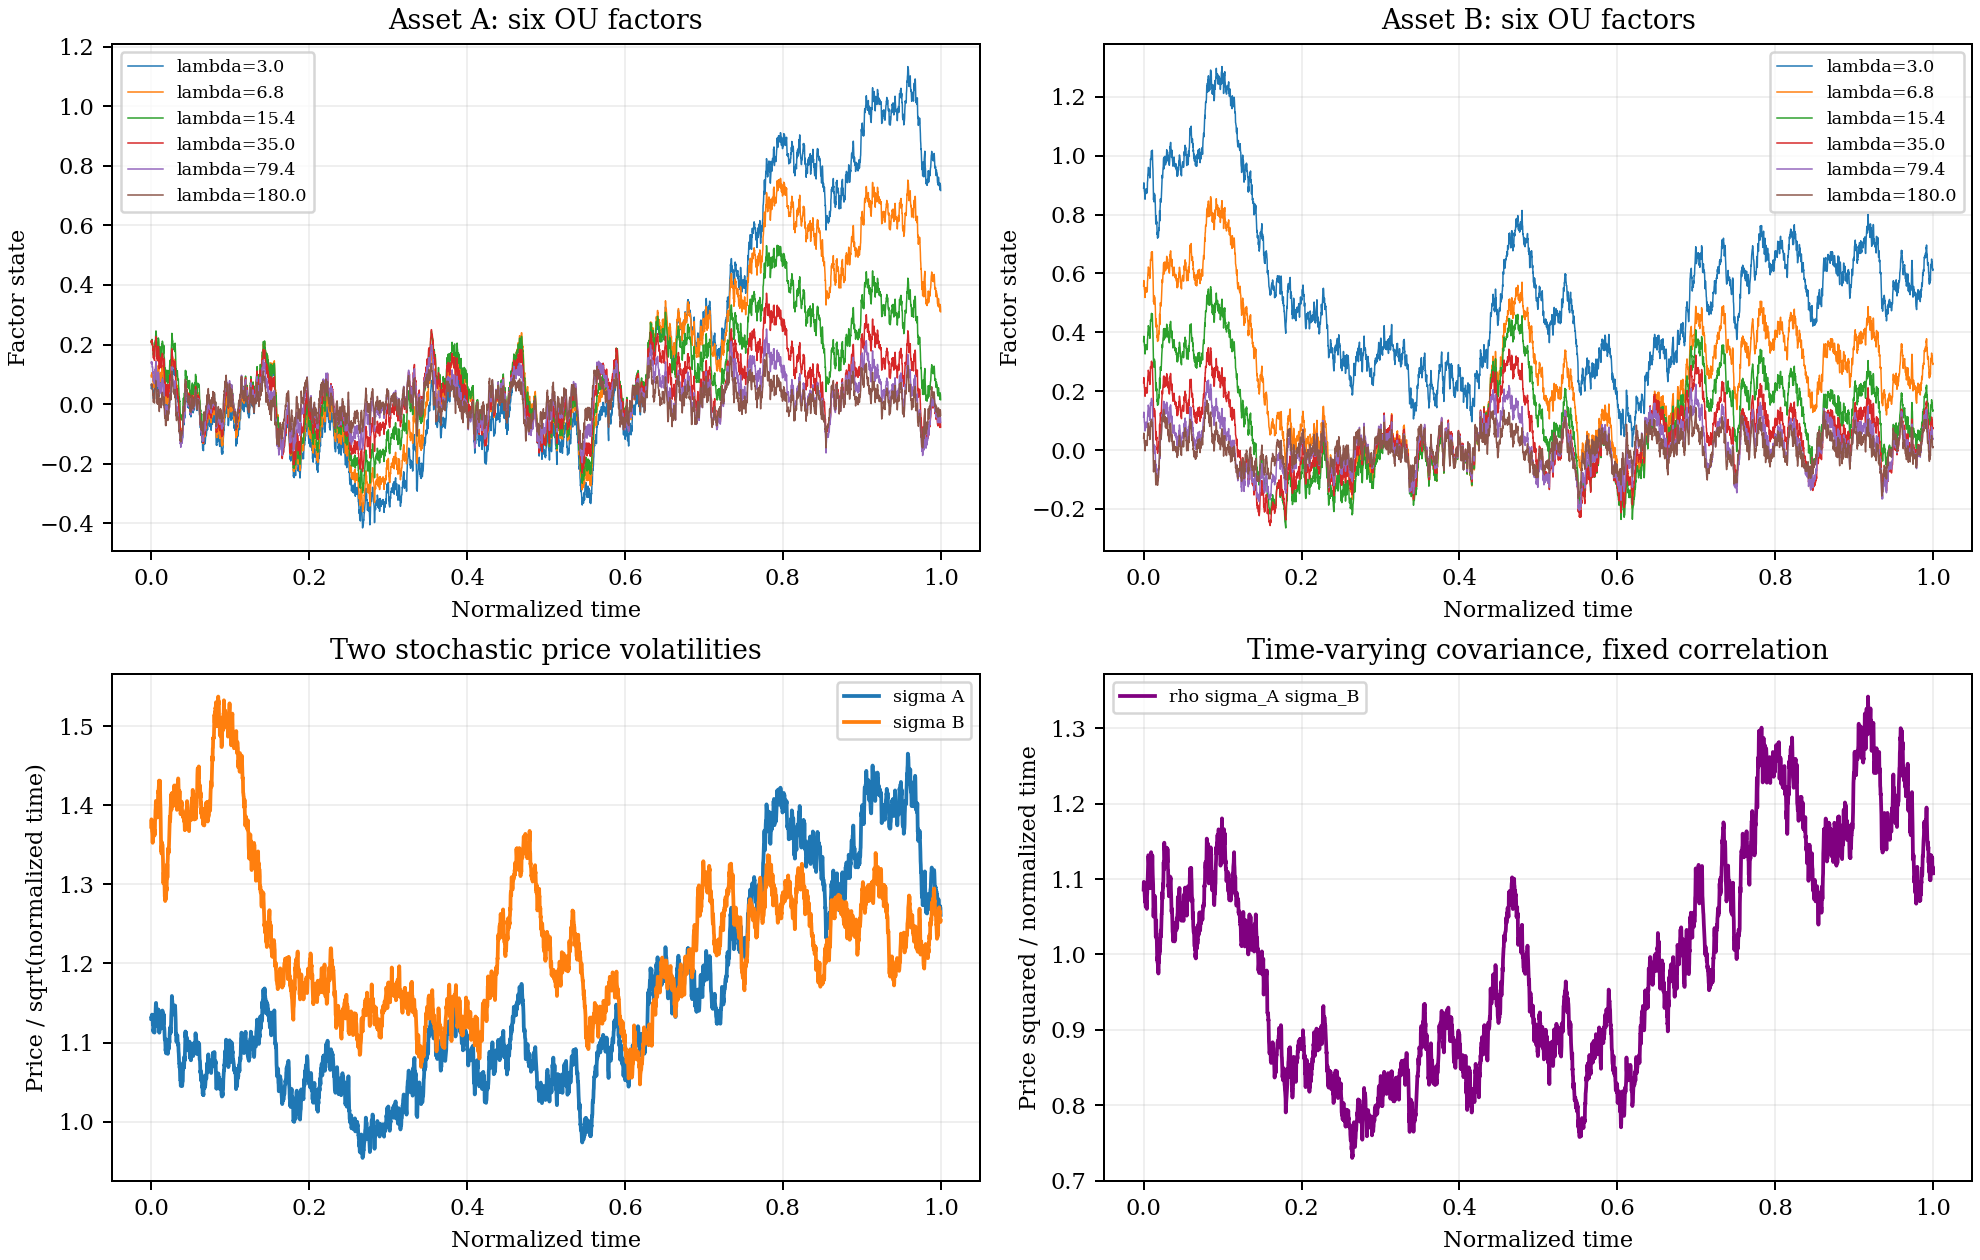
\includegraphics[width=\textwidth]{img/hft3-multiasset_volatility.png}
\caption{Two assets with six volatility factors each. Top panels show the two lifts; bottom panels show their distinct price volatilities and $\Sigma_{AB}=\rho\sigma_A\sigma_B$. Seed 73, path zero, stationary initial factor distribution, 3900 time intervals. Equal marginal parameters do not imply equal realized volatility paths.}
\label{hft3-fig:multi-vol}
\end{figure}

Exact innovations for the twelve-dimensional lift use
\[
 Q_{(i,m),(j,n)}=\nu_{ij}
 \frac{1-e^{-(\lambda_m+\lambda_n)\Delta t}}{\lambda_m+\lambda_n},
 \qquad \nu_{AA}=\nu_{BB}=1,\quad \nu_{AB}=0.35.
\]
The covariance is nearly singular for small steps. A spectral factorization removes only negative eigenvalues attributable to rounding, with a guard against a materially indefinite matrix. The maximum reconstruction discrepancy in the main run is $9.76\times10^{-19}$. This validates the factorization arithmetic, not the complete simulation discretization.

\subsection{How another asset's inventory changes a quote}
The variance rate of marked portfolio wealth is
\[
 \mathcal V(q,Y)=q^\top\Sigma(Y)q
 =q_A^2\sigma_A^2+q_B^2\sigma_B^2
 +2q_Aq_B\rho\sigma_A\sigma_B.
\]
With positive correlation, opposite-sign positions make the cross term negative. A short B position can therefore offset part of a long A exposure. The relevant object is this total risk, not the absolute inventory of either asset alone. For a unit sale of B, the exact change at fixed covariance is
\[
 \mathcal V(q-e_B,Y)-\mathcal V(q,Y)
 =-2(\Sigma q)_B+\Sigma_{BB}.
\]
Consequently the next sale reduces instantaneous risk only when $(\Sigma q)_B>\Sigma_{BB}/2$. The covariance benefit does not justify unlimited shorting. Finite order size, own-asset exposure, bounds and liquidation all matter. For example, at equal unit volatilities and $\rho=0.7$, moving from $(3,0)$ to $(3,-1)$ reduces the variance rate from 9 to 5.8; moving from $(3,-6)$ to $(3,-7)$ instead increases it, even before enforcing the inventory limit.

Multi-asset quoting and computational approximations are established research directions~\cite{BergaultEvangelistaGueantVieira2022,multifactor}. To isolate the mechanism with our existing numerical baseline, start from the separable value
\[
 \theta_{\rm sep}(t,q,Y)
 =\theta_0(t,q_A,Y_A)+\theta_0(t,q_B,Y_B).
\]
It ignores cross-asset inventory risk in its quote calculation. The first explicit correction is
\[
 C_{\rm cov}(t,q,Y)=-\gamma(T-t)\Sigma_{AB}(Y)q_Aq_B,
 \qquad \theta_{\rm cov}=\theta_{\rm sep}+C_{\rm cov}.
\]
This approximates the omitted integrated cross-risk by freezing the current covariance over the remaining horizon. It is not an exact expectation of future covariance, and it does not solve the joint control problem. It vanishes at $T$, preserving the separable terminal liquidation cost.

Define $s_B=\gamma(T-t)\Sigma_{AB}q_A$. Buying one unit of B changes the correction by $-s_B$, while selling one changes it by $+s_B$. Since the unbounded optimal offset equals the zero-gain offset minus the neighboring-inventory gain, the implementation adds $s_B$ to the raw bid offset and subtracts $s_B$ from the raw ask offset, then applies the declared bounds. Asset A uses the symmetric expression $s_A=\gamma(T-t)\Sigma_{AB}q_B$. Applying the correction before clipping avoids losing the original gain when the baseline control is already at a bound.

If $q_A>0$ and $\rho>0$, the B ask can therefore move downward relative to the separate policy: the dealer accepts a lower selling price because the fill can offset portfolio exposure. Its B bid also moves downward, discouraging further purchases. This is a change relative to the separate quote, not a promise to sell below the mid-price, nor a guaranteed execution. Figure~\ref{hft3-fig:multi-shift} makes the sign change with correlation and inventory visible while holding all other inputs fixed.

\begin{figure}[htbp]
\centering
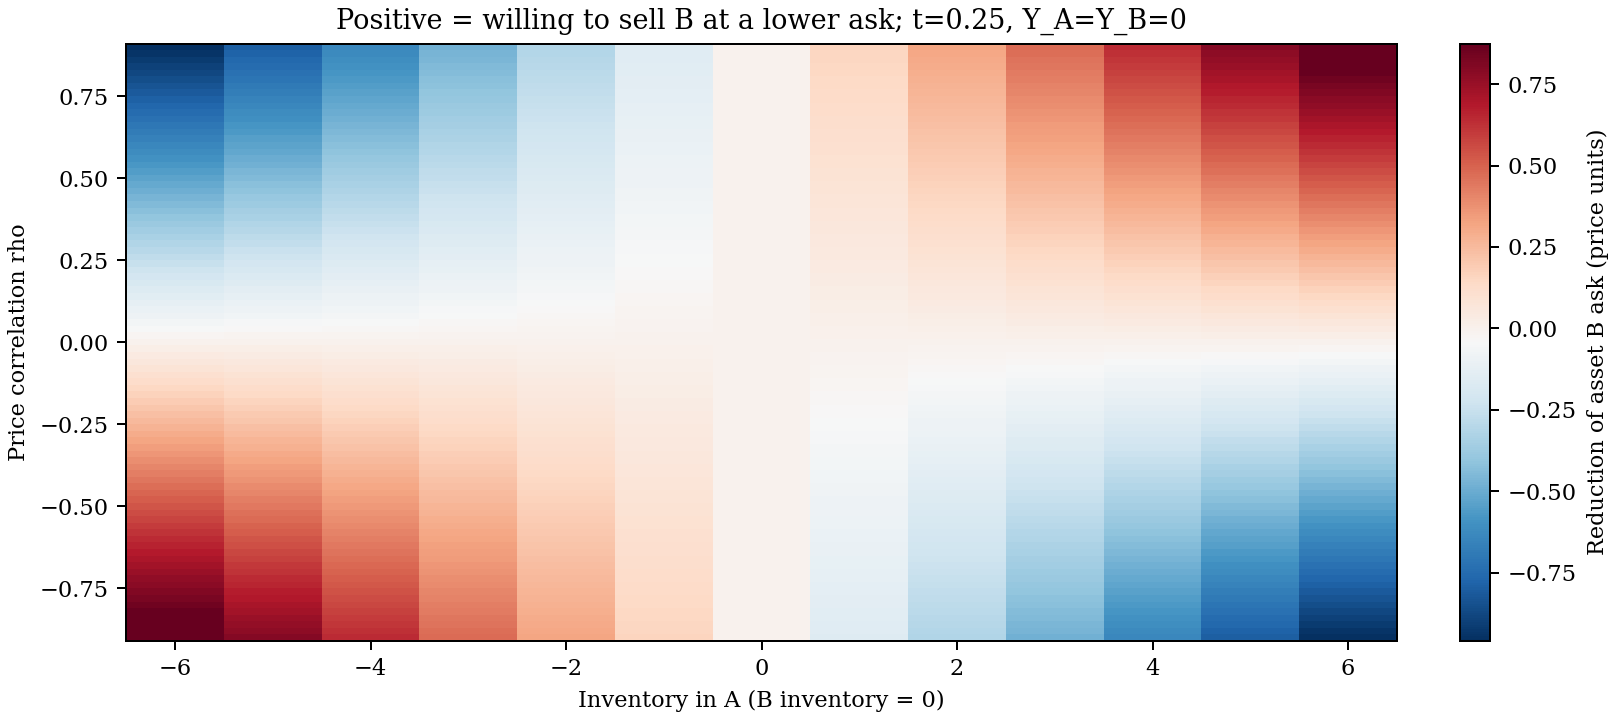
\includegraphics[width=\textwidth]{img/hft3-multiasset_quote_shift.png}
\caption{Reduction of asset B's ask relative to the separate policy, with $q_B=0$, $Y_A=Y_B=0$ and $t=0.25$. Positive values indicate a lower ask. The map varies price correlation and A inventory, using actual interpolated baseline gains and bounded controls. Zero correlation removes this explicit correction; negative correlation reverses its direction.}
\label{hft3-fig:multi-shift}
\end{figure}
\section{From a covariance proxy to a full residual correction}
The full lifted operator now has two inventory coordinates and twelve volatility coordinates. With $a$ the instantaneous covariance of the factor drivers and $\mathcal L_Z$ their OU generator, price/factor independence gives
\begin{align*}
\mathcal H[\theta]={}&\theta_t+\mathcal L_Z\theta
-\frac{\gamma}{2}(\nabla_Z\theta)^\top a\nabla_Z\theta
-\frac{\gamma}{2}q^\top\Sigma(Z)q\\
&+\sum_{i=1}^{2}\bigl[H_i(\theta(q+e_i)-\theta(q))
+H_i(\theta(q-e_i)-\theta(q))\bigr],
\end{align*}
omitting forbidden transitions. The C++ implementation supports fixed asset and total-factor dimensions and common arrival/control parameters; its caller supplies valid covariance matrices. Tests cover cross-asset risk, mixed factor Hessians, the gradient-square term and inventory bounds. In the restricted constant-covariance, no-arrival setting, the time derivative of $C_{\rm cov}$ exactly cancels the omitted cross-risk term relative to the diagonal baseline. That algebraic check does not establish cancellation in the stochastic-volatility model.

Indeed, $C_{\rm cov}$ also has factor derivatives when $\Sigma$ is stochastic, and changes all arrival Hamiltonians through the neighboring-inventory gains. Correlated volatility drivers introduce further mixed terms. The complete residual must be recomputed with these contributions before a localized fitted correction can be accepted. No residual reduction is asserted for the proxy in the experiment above.

For $N$ assets and $K$ total factors, a tensor inventory grid already contains $(2Q+1)^N$ states before discretizing volatility. Reusing separate scalar policies avoids that joint solve, but loses coupling. The explicit pair correction requires a covariance--inventory product, costing $O(N^2)$ for a dense covariance, in addition to scalar lookups; factor simulation costs are separate. This explains the proposed computational advantage and its approximation cost. No measured speedup is reported. A later fitted-policy study would require a validated multi-asset baseline and full residual to fit and test localized corrections, retaining risk, utility and computational cost as distinct acceptance criteria.
The equations now identify three errors to keep separate: approximation of memory by a finite lift, scalar compression within that lift, and numerical error in a chosen HJB solver. The numerical-methods chapter addresses the last one before the results test economic and residual effects.
